\documentclass[11pt, numbers=endperiod, parskip=half]{scrartcl}

\usepackage{graphicx}

\title{Assignment 4}
\subtitle{COS30023 - Languages in Software Development}
\author{Daniel Parker - 971328X}

\date{\today}

\begin{document}
\maketitle

\section{Problem 1}
\subsection{Finite Automaton}
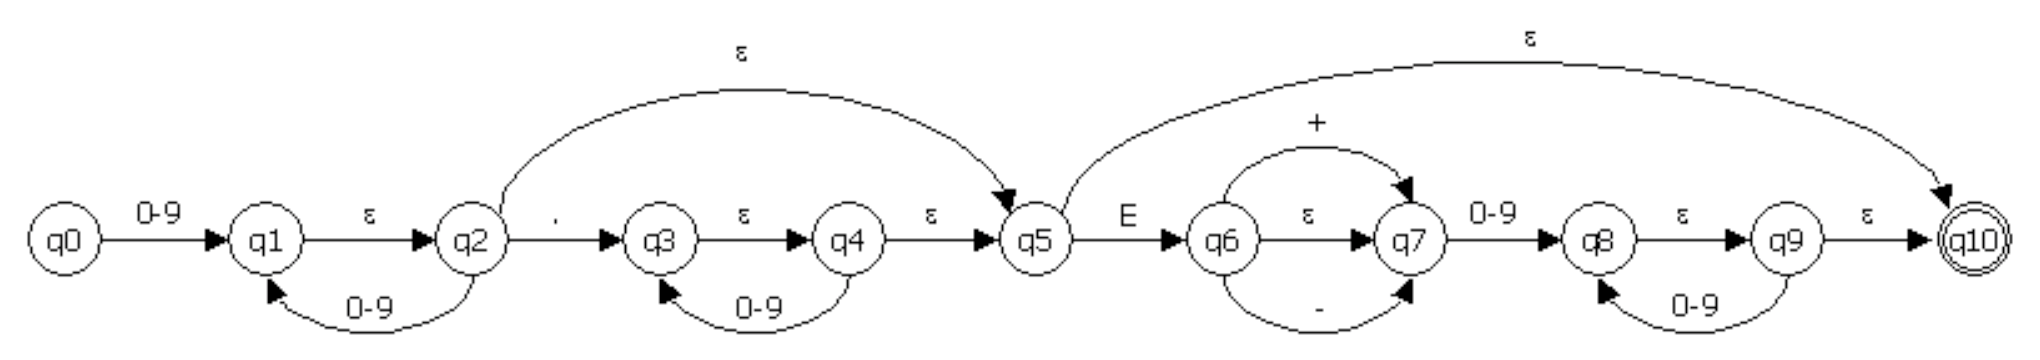
\includegraphics[scale=0.4]{automaton.png}

\subsection{Equations and Rules}
\((S_1 \cdot S_2 ) \cdot S_3 = S_1 \cdot (S_2 \cdot S_3)\)\\
\( (S_1 | S_2) \cdot T = S_1 \cdot T | S_2 \cdot T \)\\
\( T \cdot (S_1 | S_2) = T \cdot S_1 | T \cdot S_2 \)\\
\( S \cdot \epsilon = S \)\\
\( S \cdot \o = \o\)\\
\( S \cdot ( T \cdot S )^* = (S \cdot T)^* \cdot S \)

\subsection{Equation Set}
\(q_0 = 0-9 \oplus q_1\)\\
\(q_1 = \epsilon \oplus q_2\)\\
\(q_2 = 0-9 \oplus q_1\ |\ . \oplus q_3\ |\ \epsilon \oplus q_5 \)\\
\(q_3 = \epsilon \oplus q_4\)\\
\(q_4 = 0-9 \oplus q_3\ |\ \epsilon \oplus q_5\)\\
\(q_5 = E \oplus q_6\ |\ \epsilon \oplus q_{10}\)\\
\(q_6 = + \oplus q_7\ |\ - \oplus q_7\ |\ \epsilon \oplus q_7\)\\
\(q_7 = 0-9 \oplus q_8\)\\
\(q_8 = \epsilon \oplus q_9\)\\
\(q_9 = 0-9 \oplus q_8\ |\ \epsilon \oplus q_{10}\)\\
\(q_{10} = \epsilon\)
\end{document}
